\documentclass[fontsize=12pt]{article}
\usepackage[utf8]{inputenc}
\usepackage[T1]{fontenc}
\usepackage[german]{babel}
\usepackage{amsmath}
\usepackage{amsthm}
\usepackage{amsfonts}
\usepackage{amssymb}
\usepackage{minted}
\usepackage{tikz}
\usepackage{pgfplots}
\usepackage[top=2cm, bottom=2cm, left=2cm, right=2cm, headheight=1.5cm]{geometry}
\usepackage{fancyhdr}
\usepackage{mdframed}
\usemintedstyle{emacs}

\definecolor{purp}{HTML}{9A72AC}
\definecolor{re}{HTML}{FC6255}
\definecolor{gre}{HTML}{83C167}
\definecolor{blu}{HTML}{58C4DD}
\definecolor{shadecolor}{rgb}{0.85,0.85,0.85}
\definecolor{bg}{rgb}{0.95,0.95,0.95}
\setlength{\parindent}{0em} 

\BeforeBeginEnvironment{minted}{\begin{mdframed}[linewidth =2 ,backgroundcolor=bg , linecolor=black, linewidth=0.5]}
\AfterEndEnvironment{minted}{\end{mdframed}}

\newenvironment{defi}[1]{
    \begin{shaded*}
    \textbf{Definition #1} \\
}{
    \end{shaded*}
}

\newcommand{\bsp}{\textbf{Beispiel}:}
%\newcommand{\task}{\textbf{Aufgabe}:}

\newcommand{\bol}[1]{\textbf{#1}}
\newcommand{\q}[1]{\glqq #1\grqq}
\newcommand{\DODO}[1]{\textbf{\textcolor{red}{DODO:}} #1 \\ \begin{center}\includegraphics[scale=0.2]{../../media/dodo.jpg} \end{center}}

\newenvironment{task}[1]{
    \begin{shaded*}
    \textbf{Aufgabe #1}:
}{
    \end{shaded*}
}



\fancypagestyle{firstpage}{
    \setlength{\headheight}{2.5cm}
    \setlength{\footskip}{0.25cm}
    \pagestyle{fancy}
    \renewcommand{\headrulewidth}{0.4pt}
    \fancyhf{}
    \fancyhead[L]{\LARGE\textbf{Felder (arrays)}}
    \fancyhead[R]{\Large \textbf{Datum:} \hspace{2cm}}
    \fancyfoot[C]{\thepage}
}
\begin{document}
\thispagestyle{firstpage}
\setlength{\headsep}{12pt}
Es kommt häufig vor, dass in einem bestimmten Kontext nicht nur eine Variable, sondern dutzende oder hunderte gebraucht werden, um manche Dinge zu modellieren, Beispiele:
\begin{itemize}
    \item Tic-Tac-Toe-Feld, Schachbrett, allgemein: Spielfeld.
    \item Liste von Zufallszahlen. 
    \item Noten einer Klasse bei einer Arbeit, etc. 
\end{itemize}

\begin{defi}{Feld}
Ein Feld (array) ist eine Datenstruktur, in der mehrere Werte (gleichen Typs) gespeichert werden können.
\end{defi}

\textbf{Hinweise:}
\begin{itemize}
    \item Der englische Begriff \q{array} hat sich im Deutschen bereits so eingebürgert, dass außerhalb der Schule so gut wie niemand von \q{Feldern} spricht. 
    \item Streng genommen ist die Voraussetzung \q{gleicher Typ} in Java nicht immer für die Speicherung notwendig, wir beschränken uns aber zunächst darauf. 
\end{itemize}

Ein array wird wie üblich mit einer Variablen referenziert. Mit Hilfe dieser Variablen kann dann auf jeden der Einträge des Arrays zugegriffen werden, d.h. es muss nicht für jeden einzelnen Eintrag eine eigene Referenz definiert werden, dies geschieht \q{automatisch}. Zuerst muss ein array aber \textbf{initialisiert} werden. Dazu gibt es in Java zwei Möglichkeiten: 
\begin{minted}{java}
    // Ein array kann direkt durch Angabe 
    // seiner Werte in geschweiften Klammern erzeugt werden;
    int[] noten = {1,2,1,3,5,4};
    // Alternativ kann das array auch erst "leer" erzeugt werden:
    double[] groessen = new double[5];
    // So wird ein array mit 5 Einträgen erzeugt, die standardmäßig auf 0.0 gesetzt werden
\end{minted}
\begin{center}
    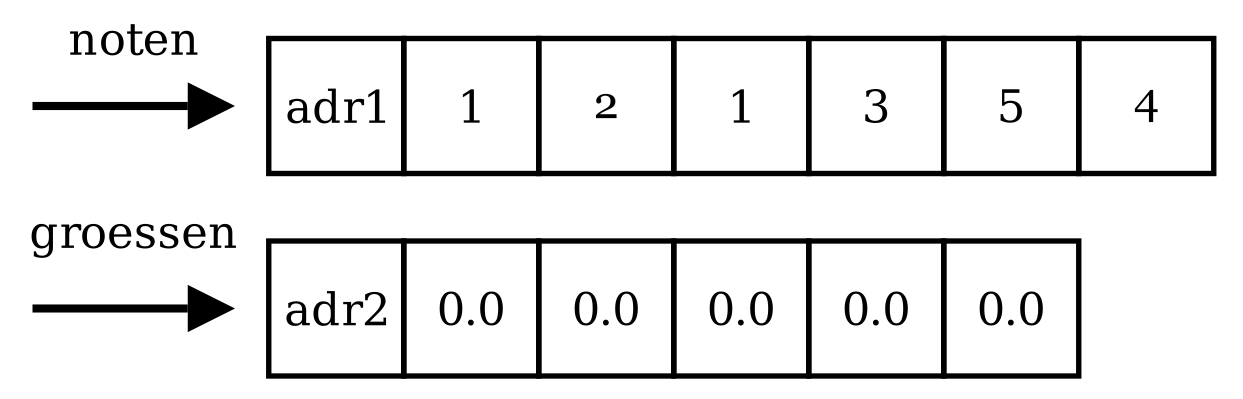
\includegraphics[scale=0.2]{media/arrays.png}
\end{center}
Die obige Darstellung ist noch nicht realitätsnah, aber dazu später mehr Details! \\

Beide Methoden können nützlich sein, je nachdem wie groß das array sein soll, bzw. ob die einzufügenden Daten bereits von Anfang an bekannt sind. \\
Will man auf einen Eintrag im array zugreifen, kann die \textbf{Klammerschreibweise} verwendet werden, z.B.:
\begin{minted}{java}
    System.out.println(noten[1]);
    // Ausgabe: 2 - das liegt daran, dass in der Informatik der erste
    // Eintrag in der Regel den Index 0 hat. 
    System.out.println(groessen[3]);
    // Ausgabe: 0.0 - möchte man dem array einen neuen Wert zuweisen:
    groessen[3] = 1.71;
    System.out.println(groessen[3]);
    // Ausgabe: 1.71
\end{minted}
\newpage
Versucht man das array insgesamt auszugeben, so stößt man zunächst auf eine rätselhafte Ausgabe: 
\begin{minted}{java}
    System.out.println(groessen);
    // Ausgabe (z.B.): [D@2f92e0f4
\end{minted}
Das liegt daran, dass die Variable \q{groessen} nur ein Zeiger ist, der zum Speicherort des arrays weist, dort werden weitere Referenzen auf die einzelnen Elemente des arrays gespeichert (dazu später mehr). Will man also ein array komplett ausgeben kann dies z.B. mit einer Wiederholung realisiert werden:
\begin{minted}{java}
    for(int i = 0; i < groessen.length; i = i+ 1) {
        System.out.println(groessen[i]);
    }
\end{minted}
In jedem Schritt verändert sich $i$ und damit auch der Eintrag auf den zugegriffen wird. Damit man nicht über das Ende \q{hinausläuft} (das würde eine Fehlermeldung produzieren) darf $i$ nur bis zum Index \q{Länge minus 1} laufen (da wir ja bei 0 anfangen!). Java bietet hier praktischerweise ein Attribut $length$ an, dass jedes array automatisch besitzt und z.B. für diesen Zweck wie oben verwendet werden kann. \\
Zusammengefasst ist die obige Wiederholung also nur eine Kurzschreibweise für folgenden Code:
\begin{minted}{Java}
    System.out.println(groessen[0]);
    System.out.println(groessen[1]);
    System.out.println(groessen[2]);
    System.out.println(groessen[3]);
    System.out.println(groessen[4]);
\end{minted}


\end{document}